\documentclass[]{beamer}

\usepackage{graphicx}% Include figure files
\usepackage{dcolumn}% Align table columns on decimal point
\usepackage{float}
\usepackage[separate-uncertainty=true,multi-part-units=single]{siunitx}
\usepackage[english]{babel}
\usepackage[]{natbib}



\title{Asteroseismology of KIC 7107778: a binary comprising almost identical subgiants}
\author{Miles Lucas}
\institute{Department of Physics and Astronomy \\ Iowa State University}

%\usetheme{lucid}
\begin{document}
	\frame {
		\titlepage
	}
	\frame {
		\frametitle{Introduction}
		Binary systems provide a good laboratory for studying stellar evolution due to their convenient constraints on metal abundance and age. Asteroseismology allows new ways to study binaries that previously could not due to being unresolved or non-eclipsing. The study of KIC 7107778 by Li and Bedding shows the power of asteroseismology in a very unique binary system. 
	}
	\frame {
		\frametitle{Asteroseismology}
		Asteroseismology is the study of how stars' brightness fluctuates. These fluctuations can be attributed to many different mechanics within stars. To analyze the periodicities we use Fourier transforms to view the data in frequency space.
	}
	\frame{
		\frametitle{KIC 7107778}
		Interesting features of this binary system
		\begin{itemize}
			\item Unresolved
			\item Widely separated
			\item Non-eclipsing
			\item Solar like oscillations from both components
		\end{itemize}	
	}
	\frame {
		\frametitle{Power Spectrum}
		\begin{figure}
			\centering
			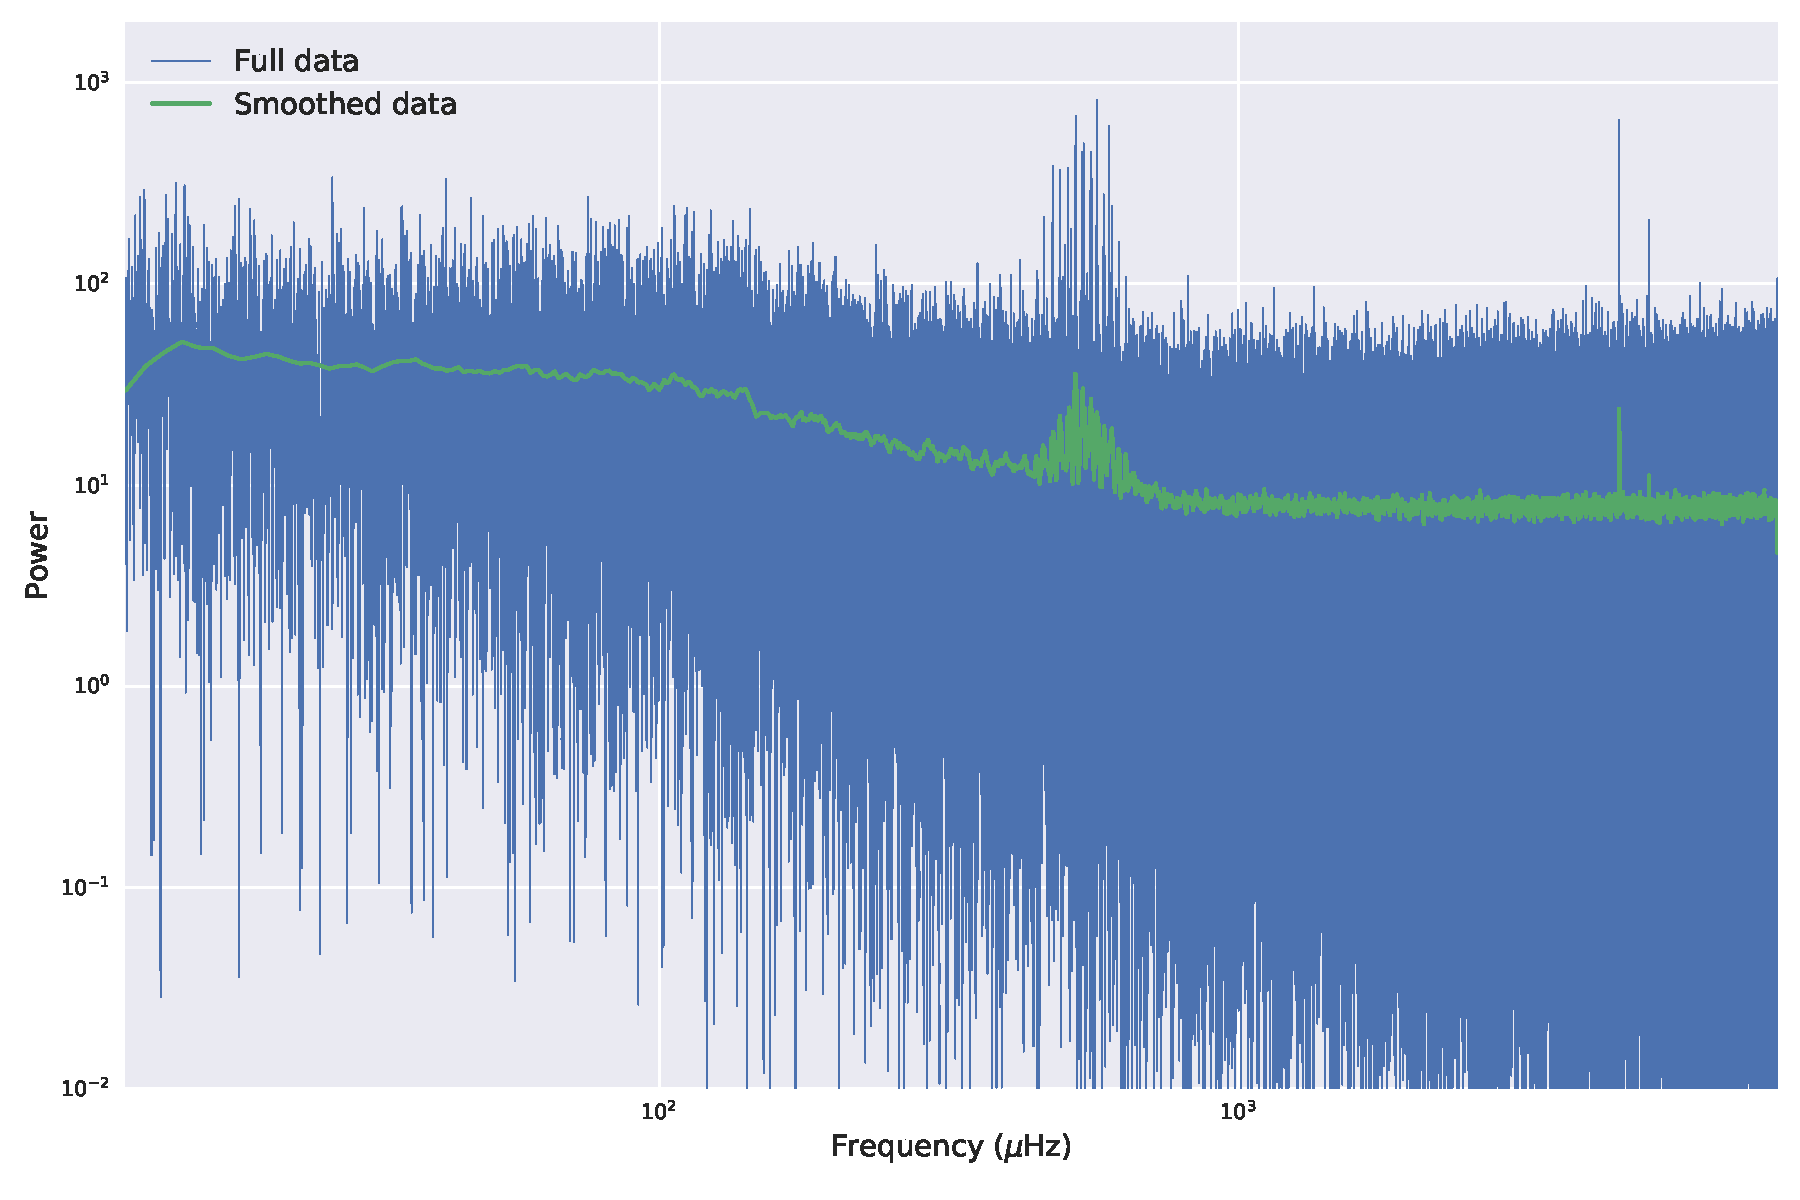
\includegraphics[width=\linewidth]{../figs/psd_pre}
		\end{figure}
	}
	\frame{
		\frametitle{Analysis Strategy}
		\begin{enumerate}
			\item Model the Gaussian envelope
			\item Analyze envelope and determine modes of interest
			\item Model the oscillation modes
		\end{enumerate}
	}
	\frame{
		\frametitle{Envelope Model}
			\begin{equation}
			P(\nu) = W + R(\nu) \left[\sum_{i=0}^{k}{H_i(\nu)} + \frac{H_0^2}{\sigma} \exp \left\lbrace  -\frac{(\nu-\nu_{max}^2)}{2\sigma^2}\right\rbrace  \right]
			\end{equation}
			where
			$$ R(\nu) = \text{sinc}^2\left( \frac{\pi \nu}{2\nu_{Nyq}}\right) $$
			and
			$$ H_i(\nu)=\frac{2\sqrt{2}}{\pi} \frac{a^2_i/b_i}{1+(\nu/b_i)^4} $$
			This is a flat noise plus response function modulating three Harvey power profiles and a Gaussian envelop.
	}

	\frame{
		\frametitle{Envelope priors}
		$$ W \sim N(12, \sigma=5) $$
		$$ a_i \sim N([59, 67, 76], \sigma=20) $$
		$$ b_i \sim N([5, 150, 400], \sigma=[10, 50, 100]) $$
		$$ H_0 \sim N(17, \sigma=5) $$
		$$ \nu_{max} \sim N(568, \sigma=5) $$
		$$ \sigma \sim Cauchy(55, 10) $$
	}
	
	\frame{
		\frametitle{Envelope posteriors}
		\begin{table}
			\centering
			\caption{Posterior Parameters}
			\label{envpost}
			\begin{tabular}[\linewidth]{llllll}
				\hline
				           &                   & mean   & sd       & 2.5    & 97.5   \\ \hline\hline
				$a_0$      & $[ppm]$           & 15.15  & 0.4591   & 14.28  & 16.07  \\ 
				$a_1$      & $[ppm]$           & 60.96  & 0.3549   & 60.29  & 61.66  \\ 
				$a_2$      & $[ppm]$           & 59.23  & 0.4772   & 58.32  & 60.17  \\ 
				$b_0$      &  $[\mu Hz]$       & 29.76  & 1.641    & 26.61  & 33.00  \\ 
				$b_1$      & $[\mu Hz]$        & 146.6  & 1.345    & 144.0  & 149.2  \\ 
				$b_2$      & $[\mu Hz]$        & 514.7  & 9.656    & 495.9  & 533.8  \\ 
				$\sigma$   &  $[\mu Hz]$       & 42.57  & 0.9466   & 40.69  & 44.40  \\ 
				$W$        &  $[ppm^2/\mu Hz]$ & 7.808  & 0.01144  & 7.786  & 7.831  \\ 
				$H_0$      & $[ppm/\mu Hz]$    & 29.82  & 0.3629   & 29.10  & 30.53  \\ 
				$\nu_{max}$&$[\mu Hz]$         & 542.2  & 0.8259   & 540.5  & 543.8  \\ 
			\end{tabular}
		\end{table}
	}

	\frame{
		\frametitle{Envelope Fit}
		
		\begin{figure}
			\centering
			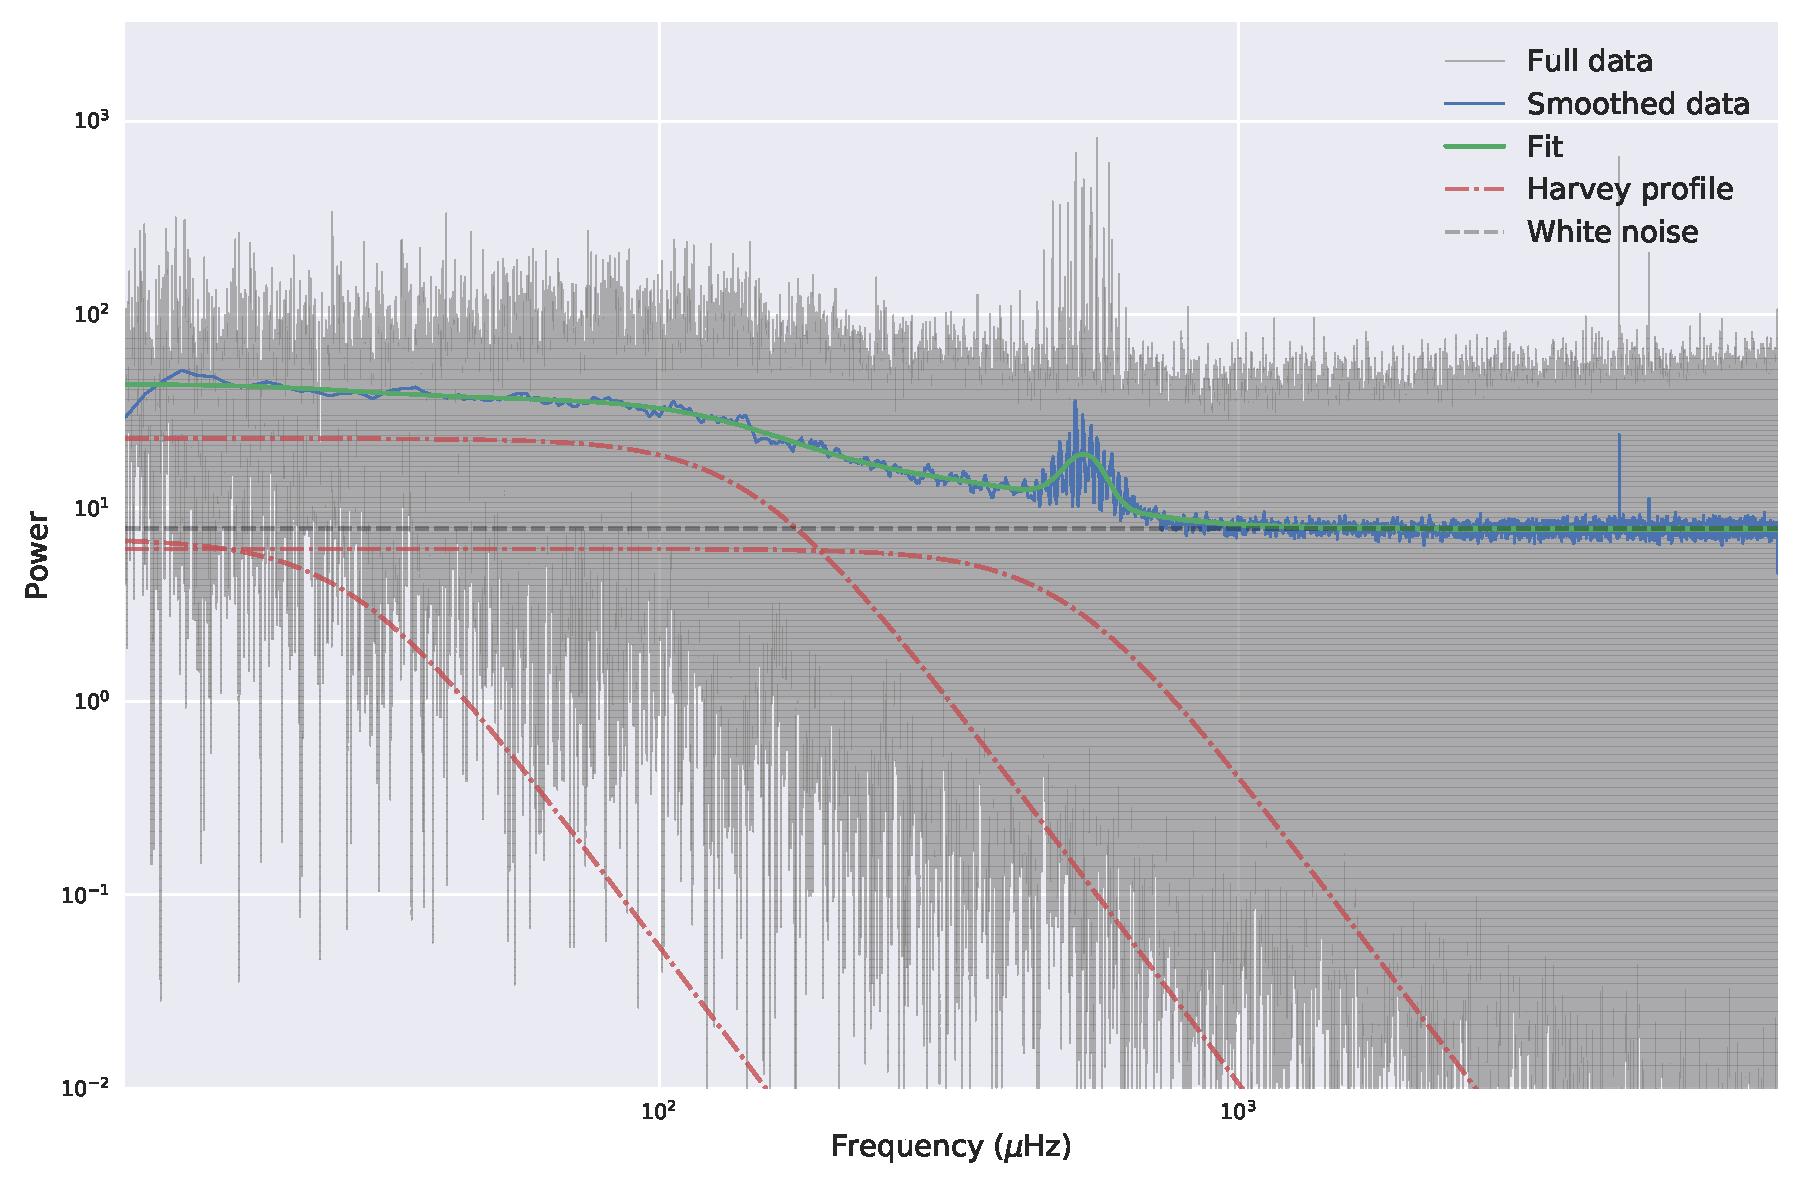
\includegraphics[width=\linewidth]{../figs/psd_fit}
		\end{figure}
	}
	\frame{
		\frametitle{Envelope Fit}
		
		\begin{figure}
			\centering
			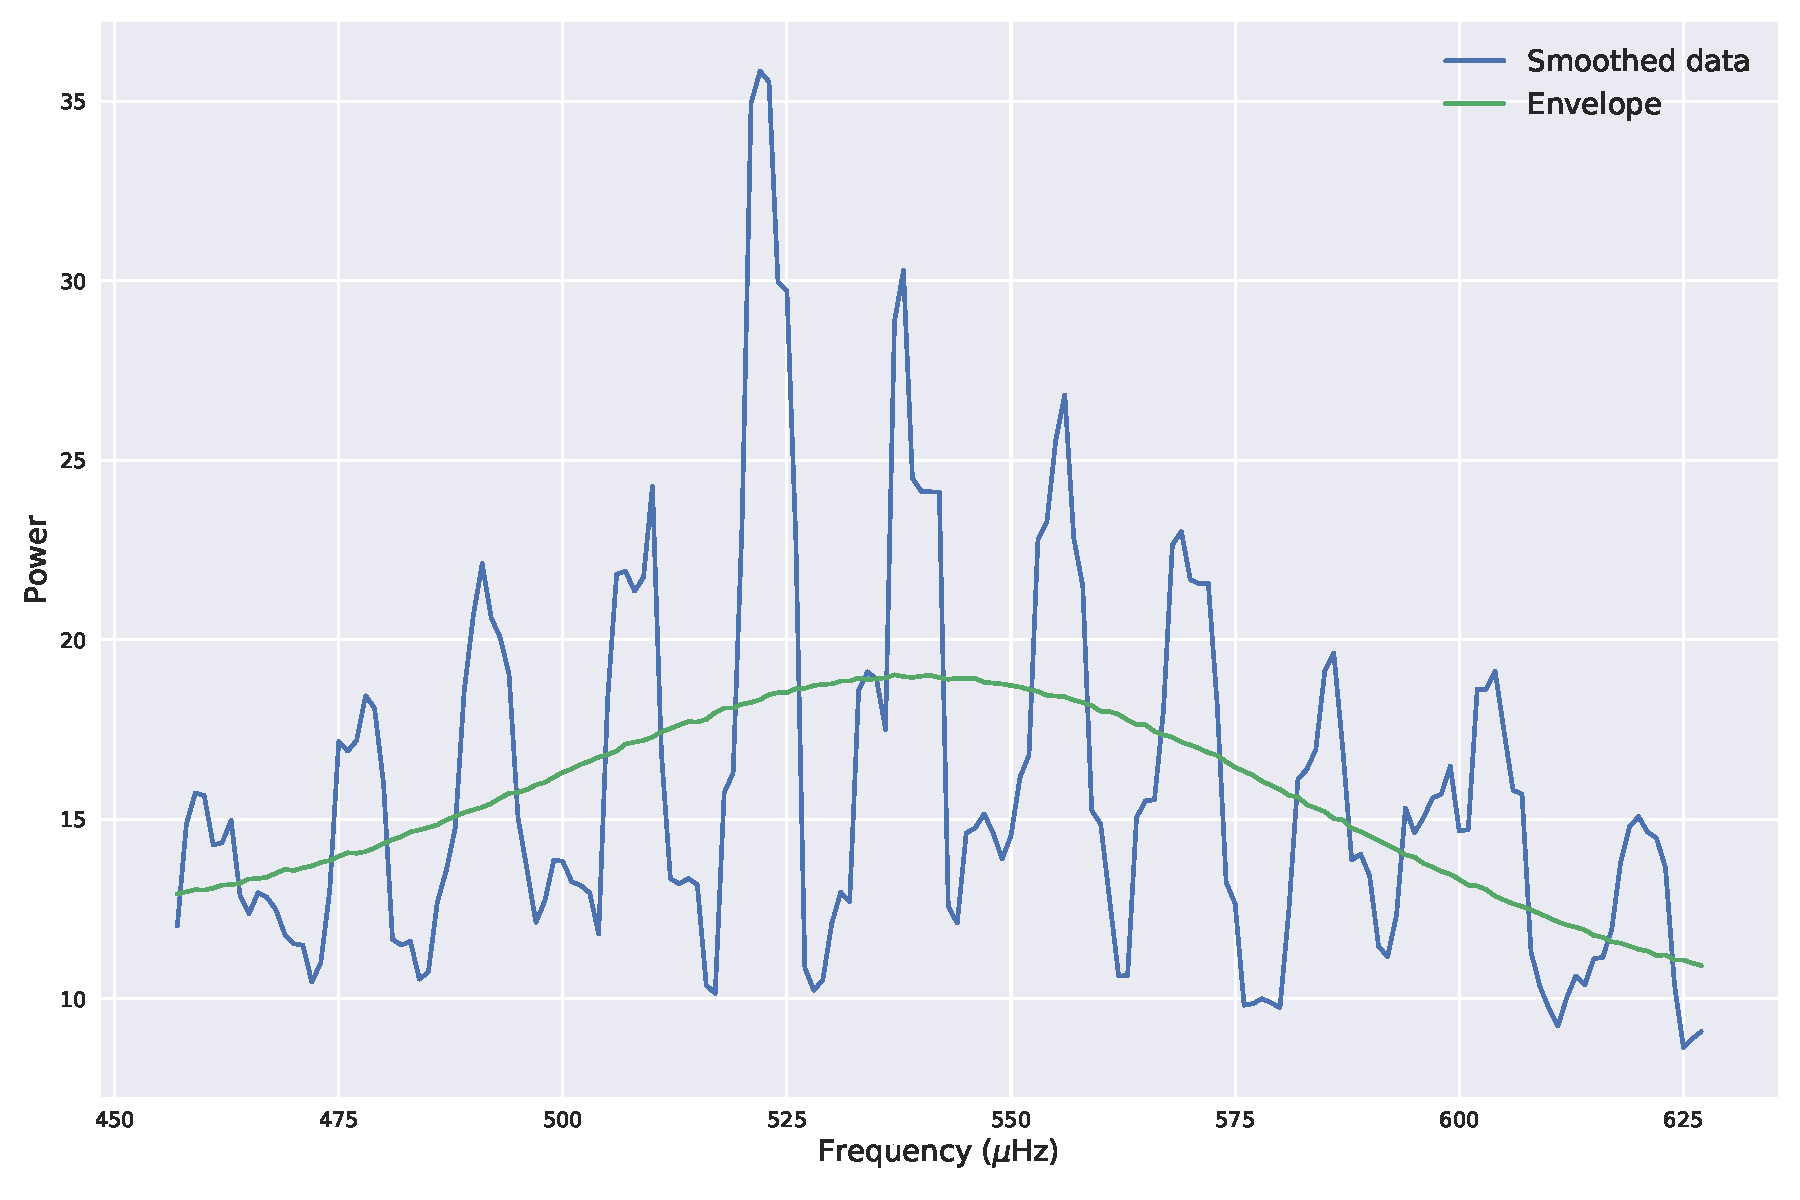
\includegraphics[width=\linewidth]{../figs/env_fit}
		\end{figure}
	}\frame{
	\frametitle{Envelope}
	
	\begin{figure}
		\centering
		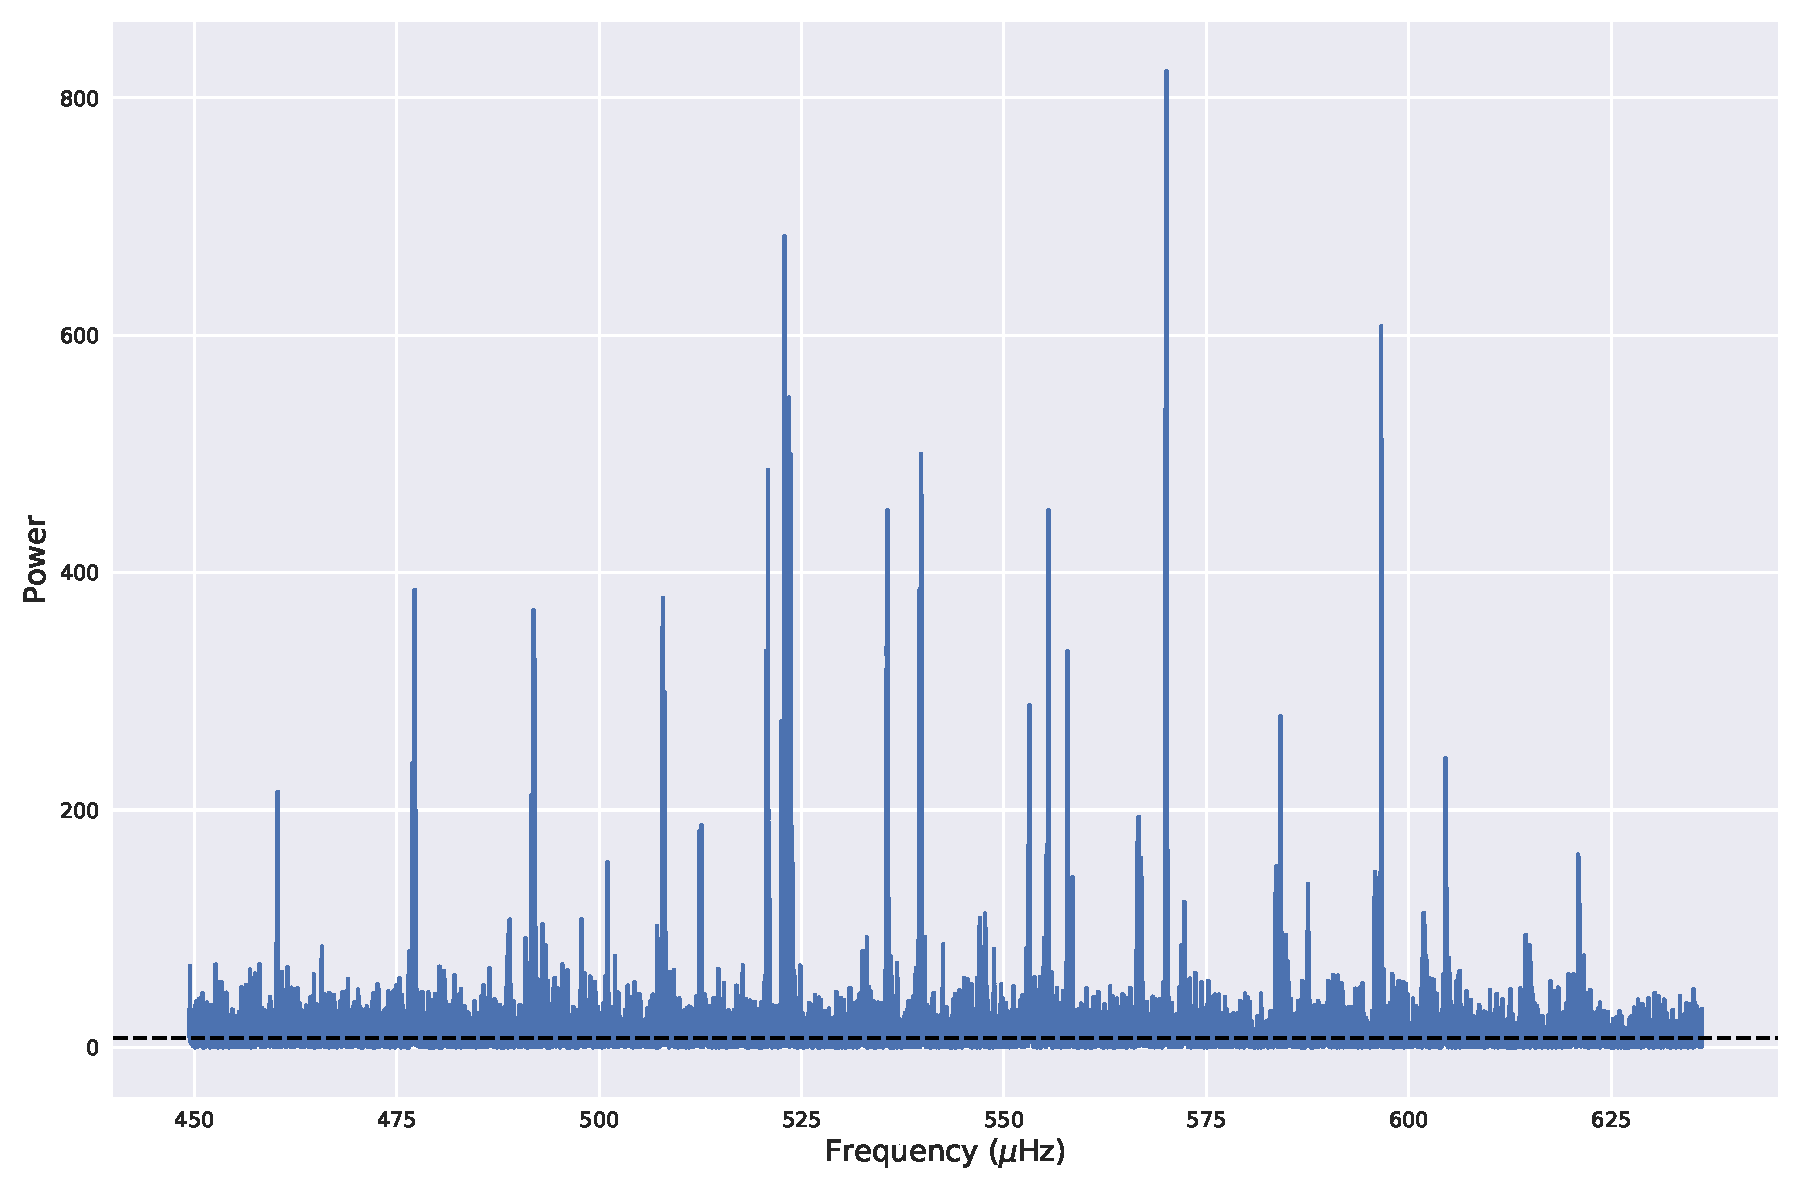
\includegraphics[width=\linewidth]{../figs/env}
	\end{figure}
	}

	\frame{
		\frametitle{Mode Model}
		\begin{equation}
		P(\nu) = R(\nu) \left[ \frac{A^2/\pi\Gamma}{1+4(\nu-\nu_0)^2/\Gamma^2} \right]
		\end{equation}
		A Lorentzian modulated by the response function.
		
	}
	\frame{
		\frametitle{Mode Model}
			\begin{figure}
				\centering
				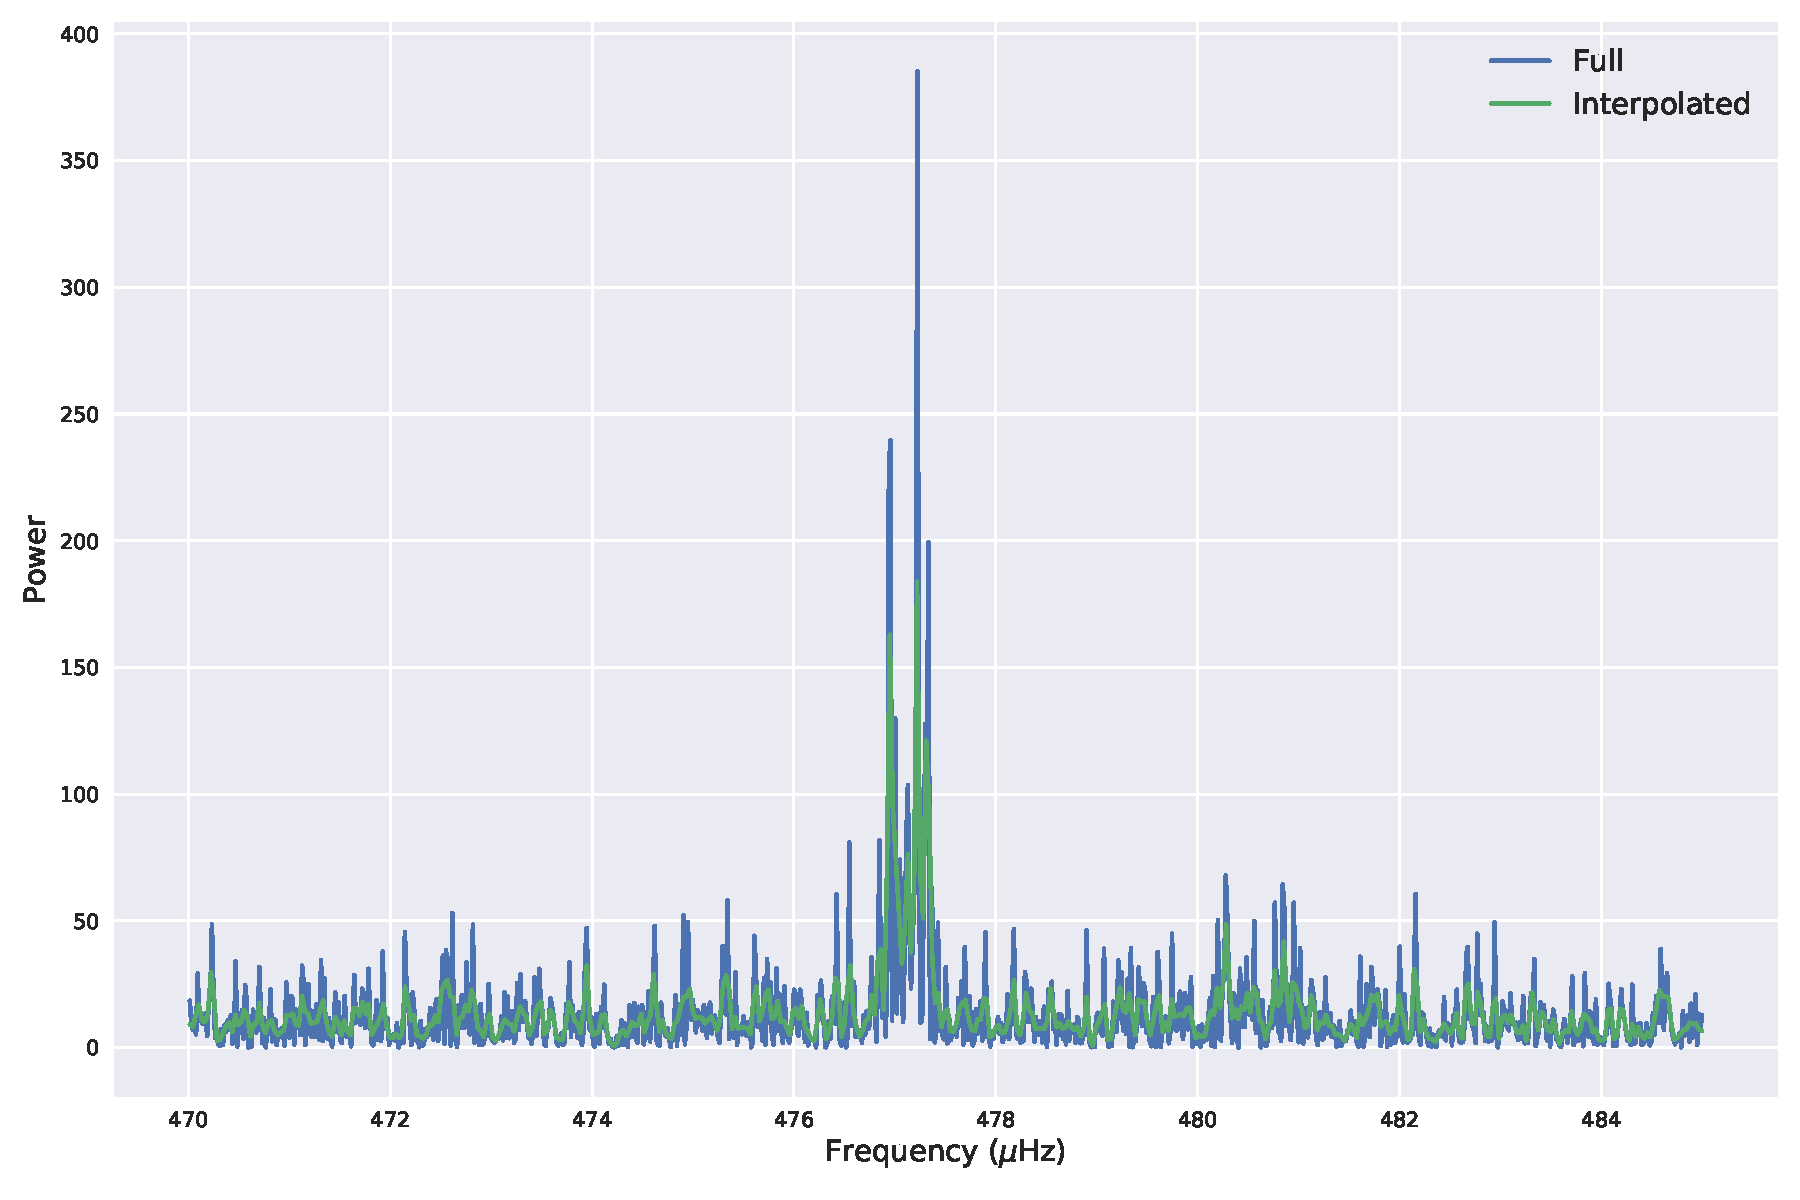
\includegraphics[width=\linewidth]{../figs/subenv}
			\end{figure}
		
	}
	\frame{
		\frametitle{Mode Model}
		$$ A \sim N(20, \sigma=10) $$
		$$ \nu_0 \sim N(477, \sigma=2) $$
		$$ \Gamma \sim \text{half-Cauchy}(2) $$		
	}
	\frame{
		\frametitle{Mode Model}
		\begin{table}
			\centering
			\caption{Posterior Parameters}
			\label{modepost}
			\begin{tabular}[\linewidth]{llllll}
				\hline
				         &                & mean   & sd      & 2.5    & 97.5   \\ \hline\hline
				$A$      & $[ppm/\mu Hz]$ & 7.480  & 0.2237  & 7.057  & 7.938  \\
				$\nu_0$  & $[\mu Hz]$     & 477.2  & 0.01817 & 477.1  & 477.2  \\
				$\Gamma$ & $[\mu Hz]$     & 0.2320 & 0.01872 & 0.1948 & 0.2684 \\
			\end{tabular}
		\end{table}		
	}
	\frame{
		\frametitle{Mode Model}
		\begin{figure}
			\centering
			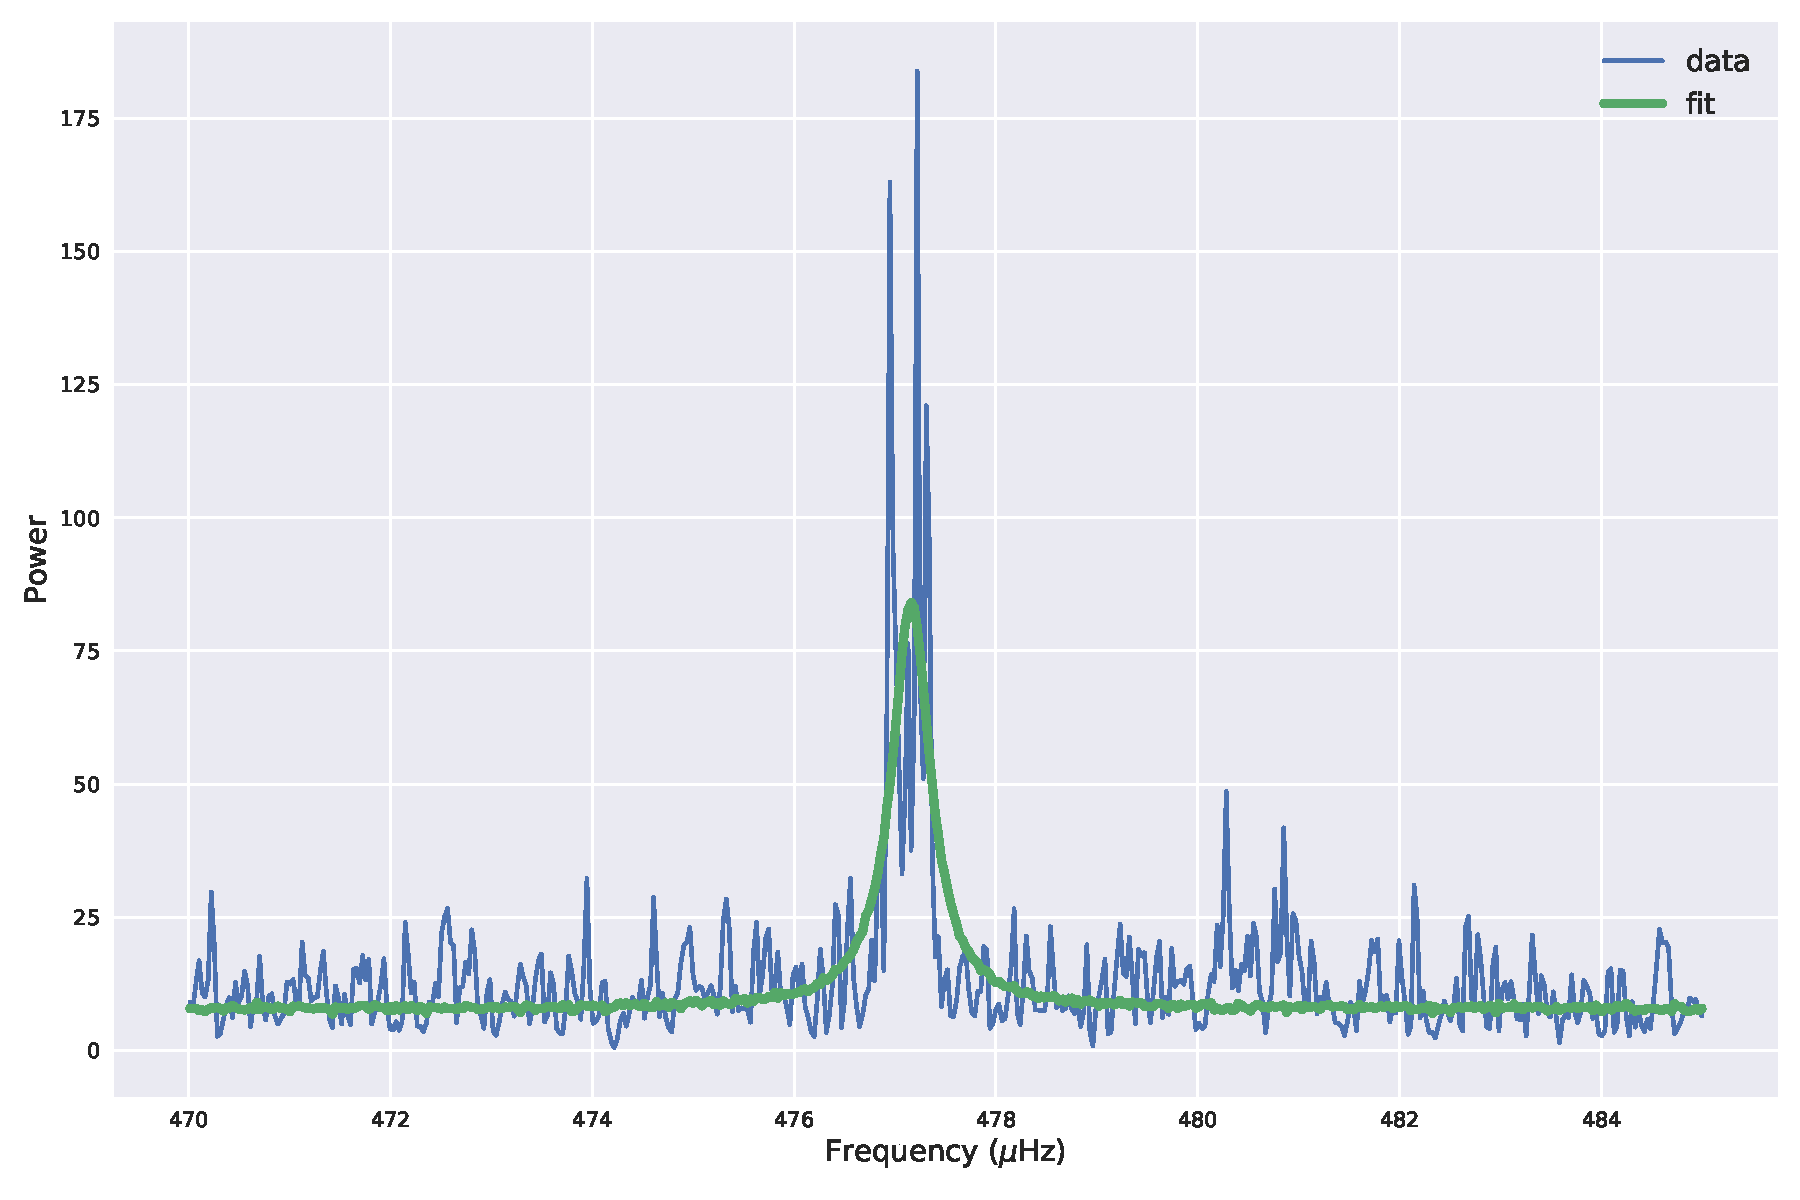
\includegraphics[width=\linewidth]{../figs/mode_fit}
		\end{figure}
		
	}

	\frame {
		\frametitle{Remarks}
		\begin{enumerate}
			\item It was a challenge to compute because of the high-dimensionality and multi-modality
			\item Authors provided no information about their priors, so I had to come up with my own
			\item Wish I could have done computations over full dataset without interpolation
		\end{enumerate}
		Special thanks to Dr. Steve Kawaler, Dr. Alicia Carriquiry, and Nicholas Berry for their assistance in this analysis.
	}

\end{document}